\documentclass[a4paper]{article}
\usepackage{geometry}
 \geometry{
 a4paper,
 total={210mm,297mm},
 left=1.25in,
 right=1.25in,
 top=1.25in,
 bottom=1.25in,
 }
\usepackage{graphicx}
\usepackage{enumitem}
%\usepackage[T1]{fontenc}
\usepackage{todonotes}
%\usepackage{graphicx}
\usepackage{pdfpages}

\begin{document}

\title{Leaf Scanner - Bussiness Model}
\author{Vikash Challa\\Preetham Sreenivas\\Sasank Chilamkurthy\\Rohith Kishan}
\date{\today}
\maketitle

\section{Problem \& Value Proposition}
\subsection{Problem Definition}
We're attempting to bridge the information gap between farmer and agricultural experts/academia using technology.


This information gap has four facets:

\begin{description}[noitemsep,topsep=0pt]
\item[Good agricultural practices]: These are academically approved set of guidelines for a crop  which will significantly improve the yields of the crop. 

Majority of farmers are usually unaware of these and still are using age old practices.
\item[Disease diagnosis \& management]: There is no widely available and reliable way for a farmer to get a disease diagnosed. 
Assuming the disease is correctly diagnosed, a majority of farmers do not know how to manage it.

\item[Preventive measures based on weather forecast]: Before hand information about untimely rains, heavy winds and abnormal temperatures can facilitate the farmer to take certain measures to prevent the damage to crop. Currently, most farmers do not have access to either the weather forecast or the preventive measures.

\item[Genuine Products]: There is no trusted way for a farmer to procure genuine agri-inputs.
\end{description}



\subsection{Current Situation \& Proposed Product}
Suppose you are a farmer. You are not completely aware of the latest agricultural practices. You have found a spot on a leaf and you are concerned that it’s a disease and want to take appropriate measures to stop the outbreak. 
\begin{description}
\item[Current Scenario] If you can afford, you hire an expert to have a look. If you cannot, you take the leaf to a pesticide/insecticide dealer and ask him to suggest a pesticide/insecticide or a remedy in general. The dealer is not an expert and may not have correct information and may suggest the wrong remedy. If the remedy is wrong, then you lose a lot of time and money in this process.

\item[Proposed Solution] A mobile application wherein you can upload the picture of that leaf and using machine learning the application detects the disease, suggests remedies and provides a marketplace to buy required genuine agri-inputs. 
This application will also feed you with academically approved set of guidelines for a crop called \emph{Good Agricultural Practices} (GAP) which will significantly improve the yields of your crop which a typical farmer like you is unaware of.
You will also be fed required precautions to be taken in response to adverse weather conditions such a heavy winds, thunderstorms etc.
It will also give you access to agricultural experts working with your crop.

\end{description}

\subsection{Value Proposition}
Following is the value we propose for each of our value recepients
\subsubsection{For farmers}
\begin{itemize}
\item Easy access to agricultural knowledge base as encapsulated in Good Agricultural Practices 
\item Accurate and reliable disease recognition of the crop
\item Access to accurate disease management techniques for a given disease
\item Trusted and genuine agri-inputs available for purchase via app/phone call
\item Timely alerts on precautions against adverse weather and GAP.
\end{itemize}

\subsubsection{For Agri-input Companies}
\begin{itemize}
\item Sales lead generation
\item Providing a channel to retail their products to farmers directly
\item Estimated demand of agri-product and locations of a given crop
\item Data about current disease outbreaks and their locations which might be useful for marketing and research
\end{itemize}

%\subsection{Evaluation}

\section{Target Customers}
\subsection{Customer Segments}
These are our target customer segments: 

\begin{enumerate}
\item Farmers affiliated with producer organizations like FPOs and agri-focused NGOs
\item Large\footnote{Farmers with more than 4.5 hectares} individual farmers growing cash crops
\item Pesticide, fungicides, chemicals and other agri-input companies
\end{enumerate}

Our current product iterations are centred around farmers who are affiliated with \emph{FPOs}. An FPO (Farmer producer organisation) is a democratic, member-owned, self governing producer organisation which is promoted by the Govt of India through NABARD\footnote{National Bank for Agriculture and Rurual Development} with the vision to tackle the fragmentation problem in India.

We are currently focusing on \textbf{banana} for our MVP. This is because banana farmers are usually economically well off and have been traditionally early adopters of new agricultural technologies like tissue culture.

\subsection{Customer Profile}
Our customer farmer will have and be able to use a smartphone or will be enthusiastic to learn using an app upon minimal training.
These type of farmers usually are 
\begin{itemize}
\item Financially well-to-do
\item Literate
\item Enthusiastic to try new techniques instead of customary techniques
\item Young or middle aged
\end{itemize} 

\section{Channels}
We're going to attract our customers through FPOs and similar organizations.
We'll contact FPO managers who in turn will recommend our product to the shareholders of FPO.

Our service is mainly delivered through mobile application and possibly, phone calls.
Our customers can place orders of agri-inputs either through the app directly or phone call.

We'll take feedback through app itself and through FPO managers who will be in regular touch with farmers. 



\section{Competition}
There are a few companies like agro-star and snapdeal who are trying to bring the Indian agro-chemical market online. 
A company called Farms-n-Farmers is trying to optimize the whole vertical through face to face personal assistance. DestaMart is a B2B firm connecting agri-input producers with dealers and shop-owners. 
They also have an agricultural knowledge dissemination portal called DestaTalk.

However, we are not aware of any firm which classifies leaf images using machine learning and is trying to bridge farmer-expert information gap through technology.
Computer vision based algorithm will be our primary differentiation.

\section{Key Resources}
We need following resources to start and run our venture :
\begin{itemize}
\item Datasets of diseased leaf images
\item Distribution networks for agri-inputs
\item Agricultural expertise for GAP and most of our features
\item Machine learning and computer vision expertise for disease recognition 
\item Software engineering expertise for Android development and relevant backend
\end{itemize}

Initially, we will obtain dataset by going to farms with diseased plants and taking photos ourselves.
We will acquire distribution networks by partnering with agri-input companies and a logistics company. 
We have access to wide network of agricultural experts through our mentors. We plan to hire a few experts as consultants initially.
Founders already have significant domain knowledge of computer vision, machine learning and software development. 
We plan to get mentored by a professor at IIT Bombay with whom one of us already worked with.

\section{Revenue Model}
\subsection{Revenue Streams}
Our primary revenue is through
\begin{itemize}
\item Dealer's cut from sale of agri-inputs
\item Fee for lead generation for agri-input companies
\item Sale of relevant agricultural data to agri-input companies
\end{itemize}

\subsection{Expenses}
These will be primary expenses
\begin{description}
\item[Fixed costs]:
	\begin{itemize}
		\item Product development \& support
		\item Salaries and rents
		\item Payrolls for agricultural experts
	\end{itemize}
\item [Variable Costs]:	
	\begin{itemize}
		\item Maintenance of distribution network
		\item Customer support
		\item Marketing costs
	\end{itemize}




\end{description}

\section{Market Analysis}
Total Indian agro-chemical market is projected to be \$6.8 bn by FY2017. 

Since our initial target segment is FPO affiliated farmers, we'll give an estimate of market size of this segment. Each FPO typically consists of 500 -- 2000 registered farmers. In 2014, there were around 200 FPO's registered. The current trend suggests that there will be a minimum of 1000 FPOs by the end of 2016.

\begin{itemize}
\item[] An average FPO has 1000 farmers and it is projected that there will be about 1000 FPOs
\item[] So our total number of customers are 1000*1000.
\item[] Average cultivated land for our target customer $\sim$  5 acres (= 2 hectares)
\item[] Average investment per acre on pesticides, fungicides and other chemicals is $\sim$ 30K INR (depends on crop)
\item[] So, Market potential for a FPO based product is $1000000 \times 5 \times 30000 \times 0.15 \approx 22.5$ billion INR = \$375 million
\end{itemize}

So our initial target market size is around \$375 million. Typical margins in this industry range from 20-30\%.




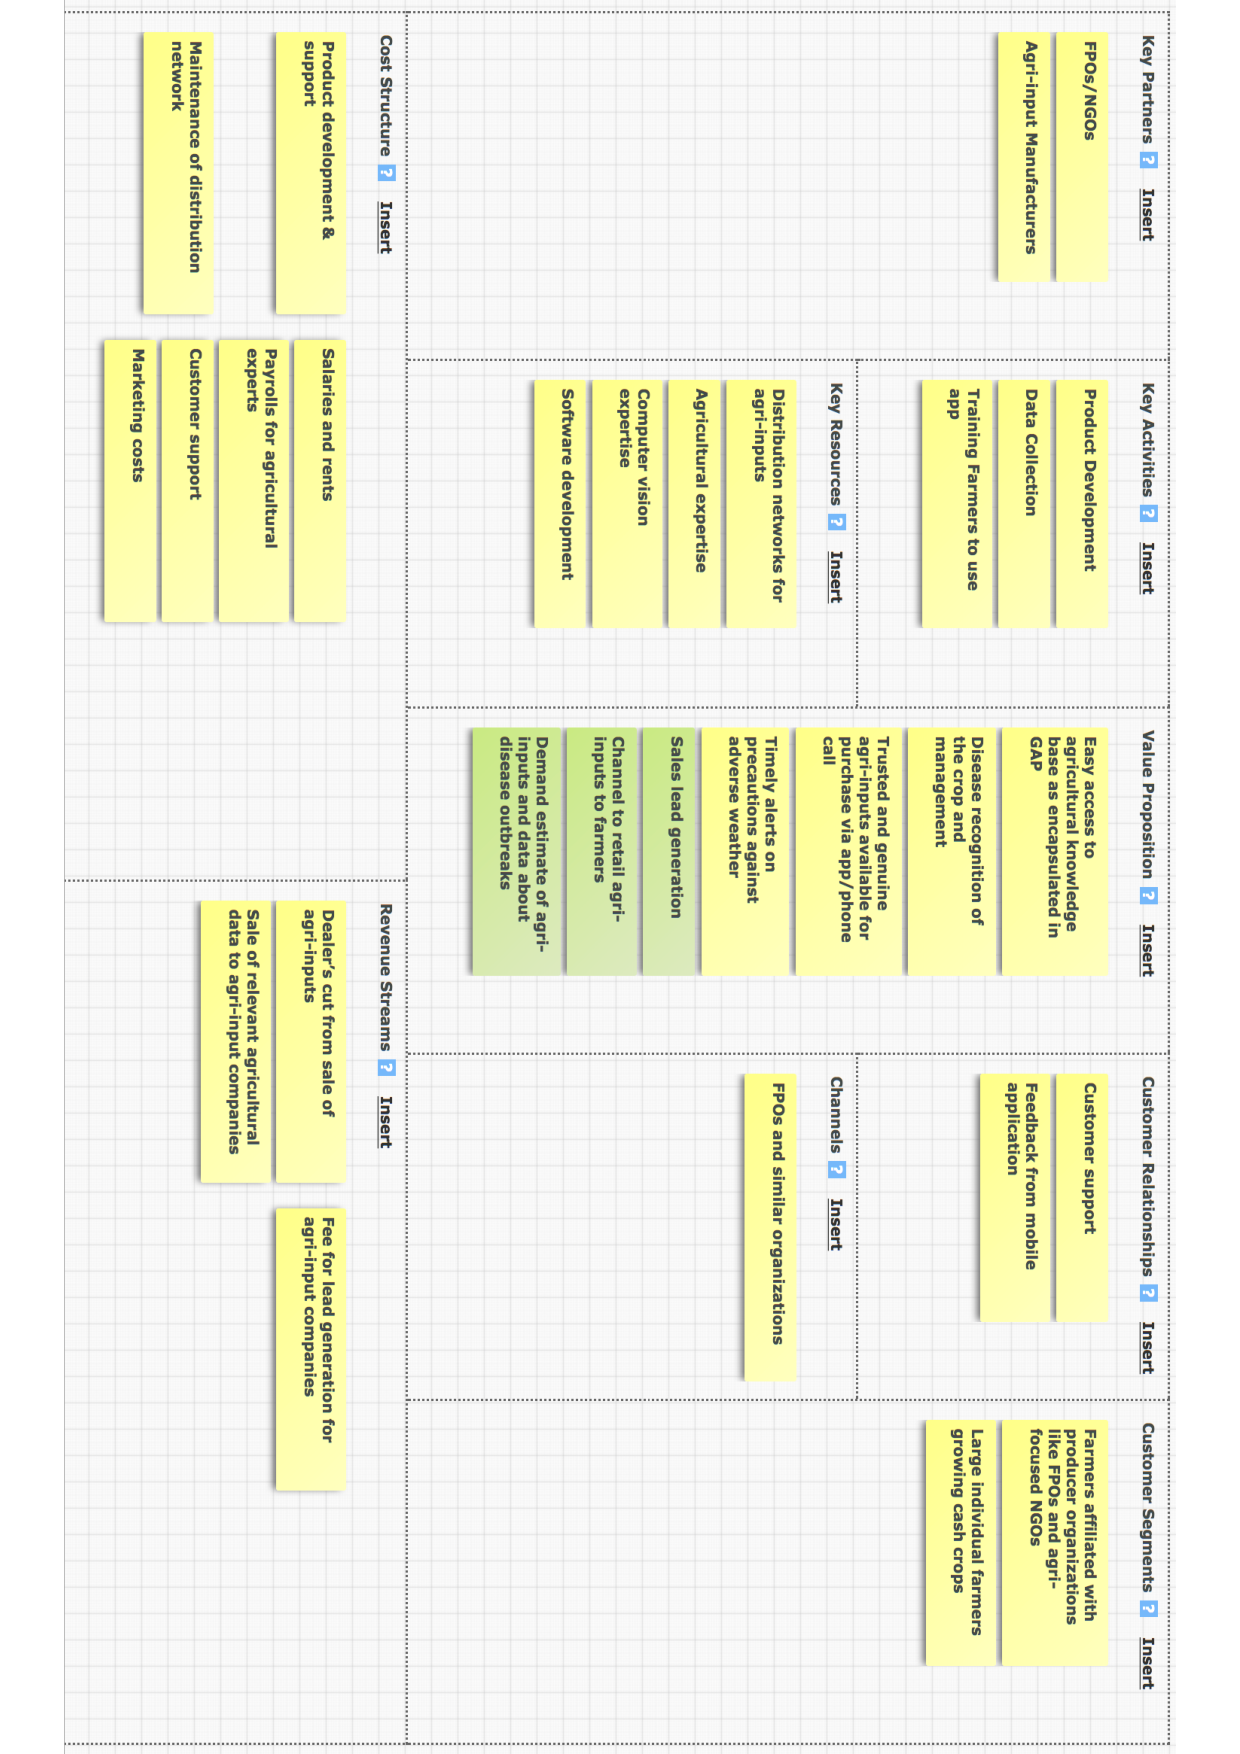
\includepdf{bmodel-canvas.pdf}
\end{document}